\section{Phân hệ Lịch sử Đơn hàng (Order History)}

\subsection{Đặc tả Use Case}
Phân hệ Lịch sử Đơn hàng cho phép khách hàng tra cứu toàn bộ các đơn hàng đã đặt trong quá khứ, theo dõi trạng thái pha chế và kiểm tra hóa đơn chi tiết. Sơ đồ Use Case được minh họa tại Hình~\ref{fig:usecase-order-history}.

\begin{figure}[htbp]
    \centering
    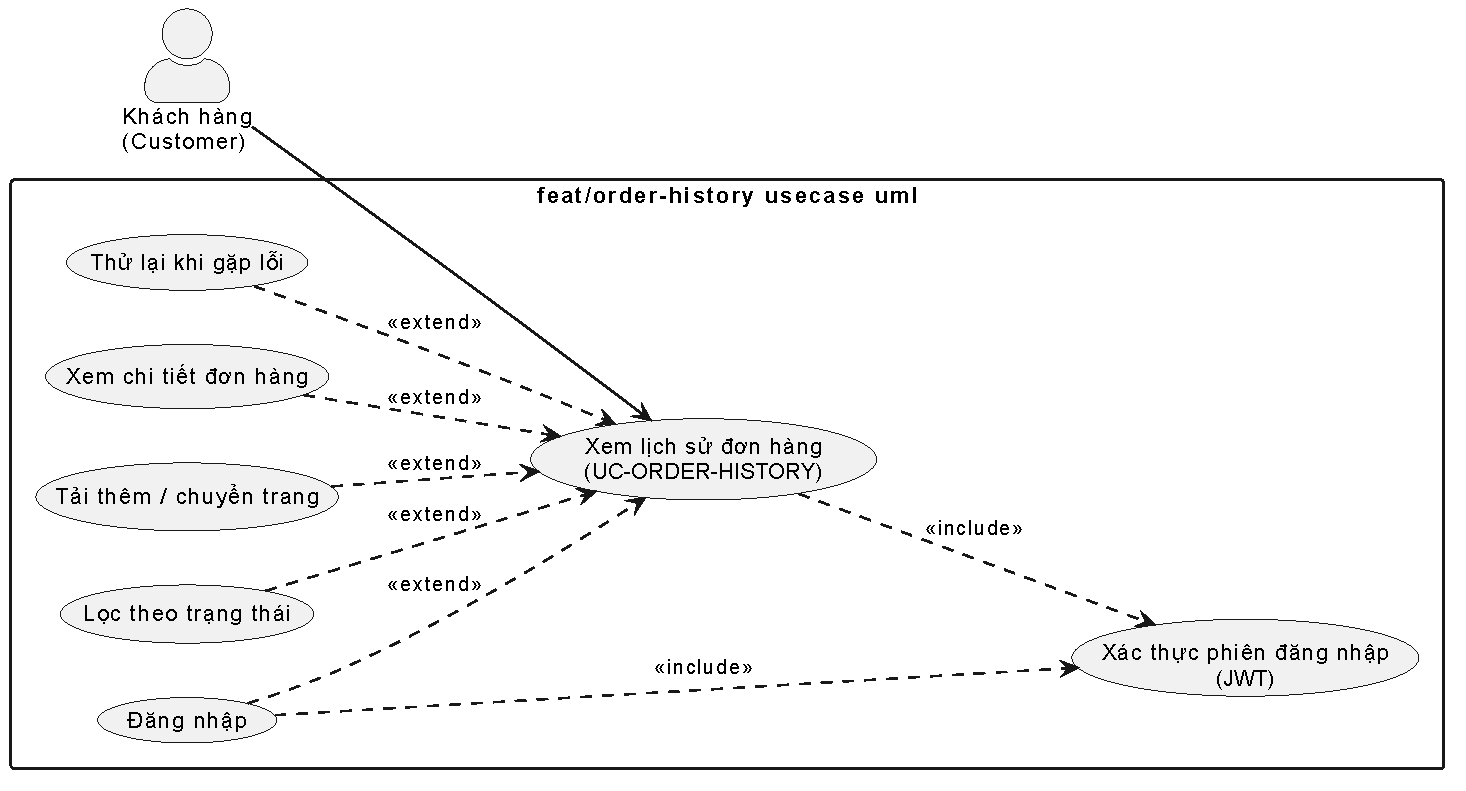
\includegraphics[width=0.75\textwidth]{figures/usecase-order-history.pdf}
    \caption{Sơ đồ Use Case - Phân hệ Lịch sử Đơn hàng}
    \label{fig:usecase-order-history}
\end{figure}

\begin{table}[htbp]
\centering
\small
\caption{Đặc tả Use Case: Tra cứu Lịch sử và Chi tiết Đơn hàng (UC-HIS-01)}
\label{tab:uc-spec-history}
\begin{tabularx}{\textwidth}{p{2.8cm}X}
\toprule
\textbf{Mục} & \textbf{Chi tiết Đặc tả} \\
\midrule
\textbf{Actor} & Khách hàng đã đăng nhập \\
\midrule
\textbf{Tiền điều kiện} & Khách hàng đã đăng nhập vào hệ thống. \\
\midrule
\textbf{Hậu điều kiện} & Danh sách các đơn hàng và trạng thái chi tiết hiển thị trực quan. \\
\midrule
\textbf{Luồng chính} & 
1. Khách hàng nhấp vào mục "Lịch sử đơn hàng" trên thanh điều hướng hoặc truy cập \texttt{/orders}.\newline
2. Giao diện gửi request \texttt{GET /api/v1/orders} kèm Bearer Token.\newline
3. Backend truy vấn các đơn hàng thuộc về \texttt{userId} hiện tại, sắp xếp giảm dần theo thời gian tạo (\texttt{createdAt desc}).\newline
4. Màn hình hiển thị danh sách các thẻ đơn hàng: mã hiển thị \texttt{\#orderNumber}, ngày giờ đặt, tổng tiền, huy hiệu trạng thái (ví dụ "Đã thanh toán", "Đã hủy").\newline
5. Khách hàng nhấp vào một đơn hàng để xem chi tiết hóa đơn (\texttt{/orders/[id]}): danh sách từng món, size, topping, số tiền giảm giá và phương thức thanh toán. \\
\midrule
\textbf{Luồng ngoại lệ} & 
- Người dùng chưa có đơn hàng nào: Giao diện hiển thị thông báo "Bạn chưa có đơn hàng nào" và nút liên kết "Bắt đầu đặt món".\newline
- Phiên đăng nhập hết hạn: Báo lỗi \texttt{401 Unauthorized}, tự động chuyển hướng về trang đăng nhập. \\
\bottomrule
\end{tabularx}
\end{table}

\subsection{Sơ đồ Hoạt động (Activity Diagram)}
Quy trình truy vấn danh sách và xem chi tiết trạng thái đơn hàng được thể hiện tại Hình~\ref{fig:activity-order-history}.

\begin{figure}[htbp]
    \centering
    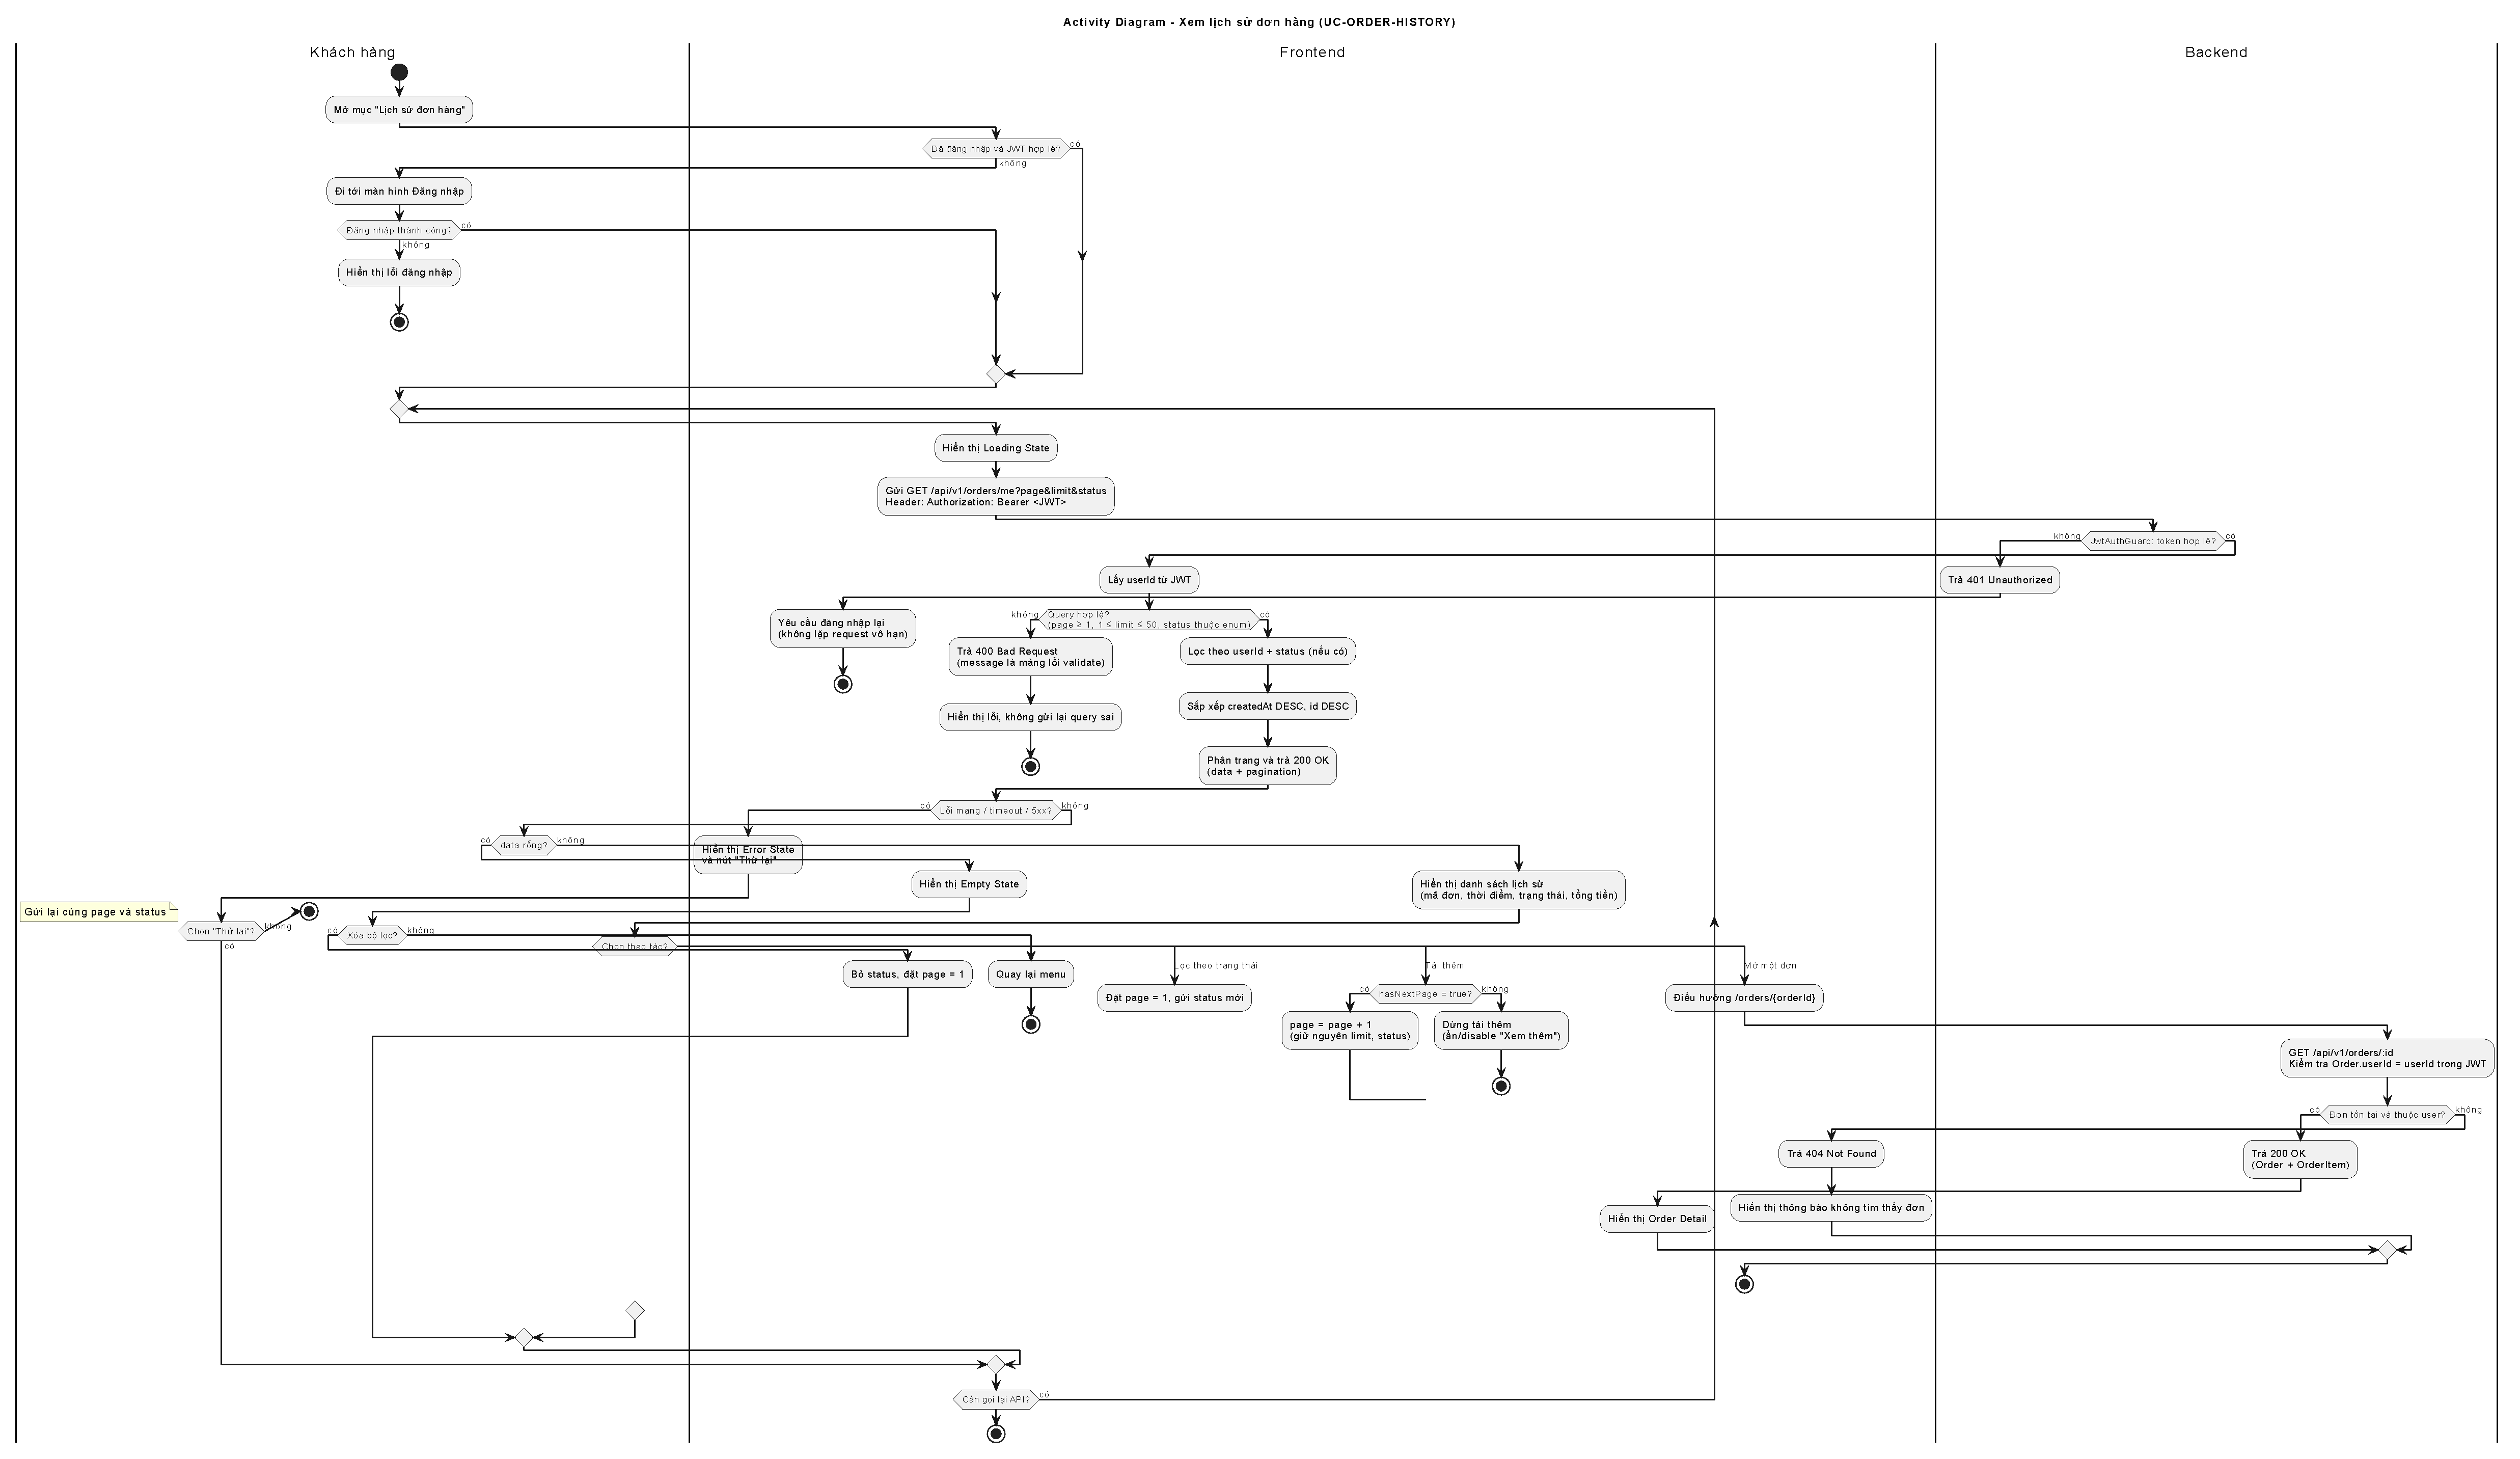
\includegraphics[width=0.75\textwidth]{figures/activity-order-history.pdf}
    \caption{Sơ đồ Hoạt động - Phân hệ Lịch sử Đơn hàng}
    \label{fig:activity-order-history}
\end{figure}

\subsection{Sơ đồ Tuần tự (Sequence Diagram)}
Sơ đồ Tuần tự minh họa tương tác nạp dữ liệu lịch sử đơn hàng từ Frontend đến Controller, Service và Prisma tại Hình~\ref{fig:sequence-order-history}.

\begin{figure}[htbp]
    \centering
    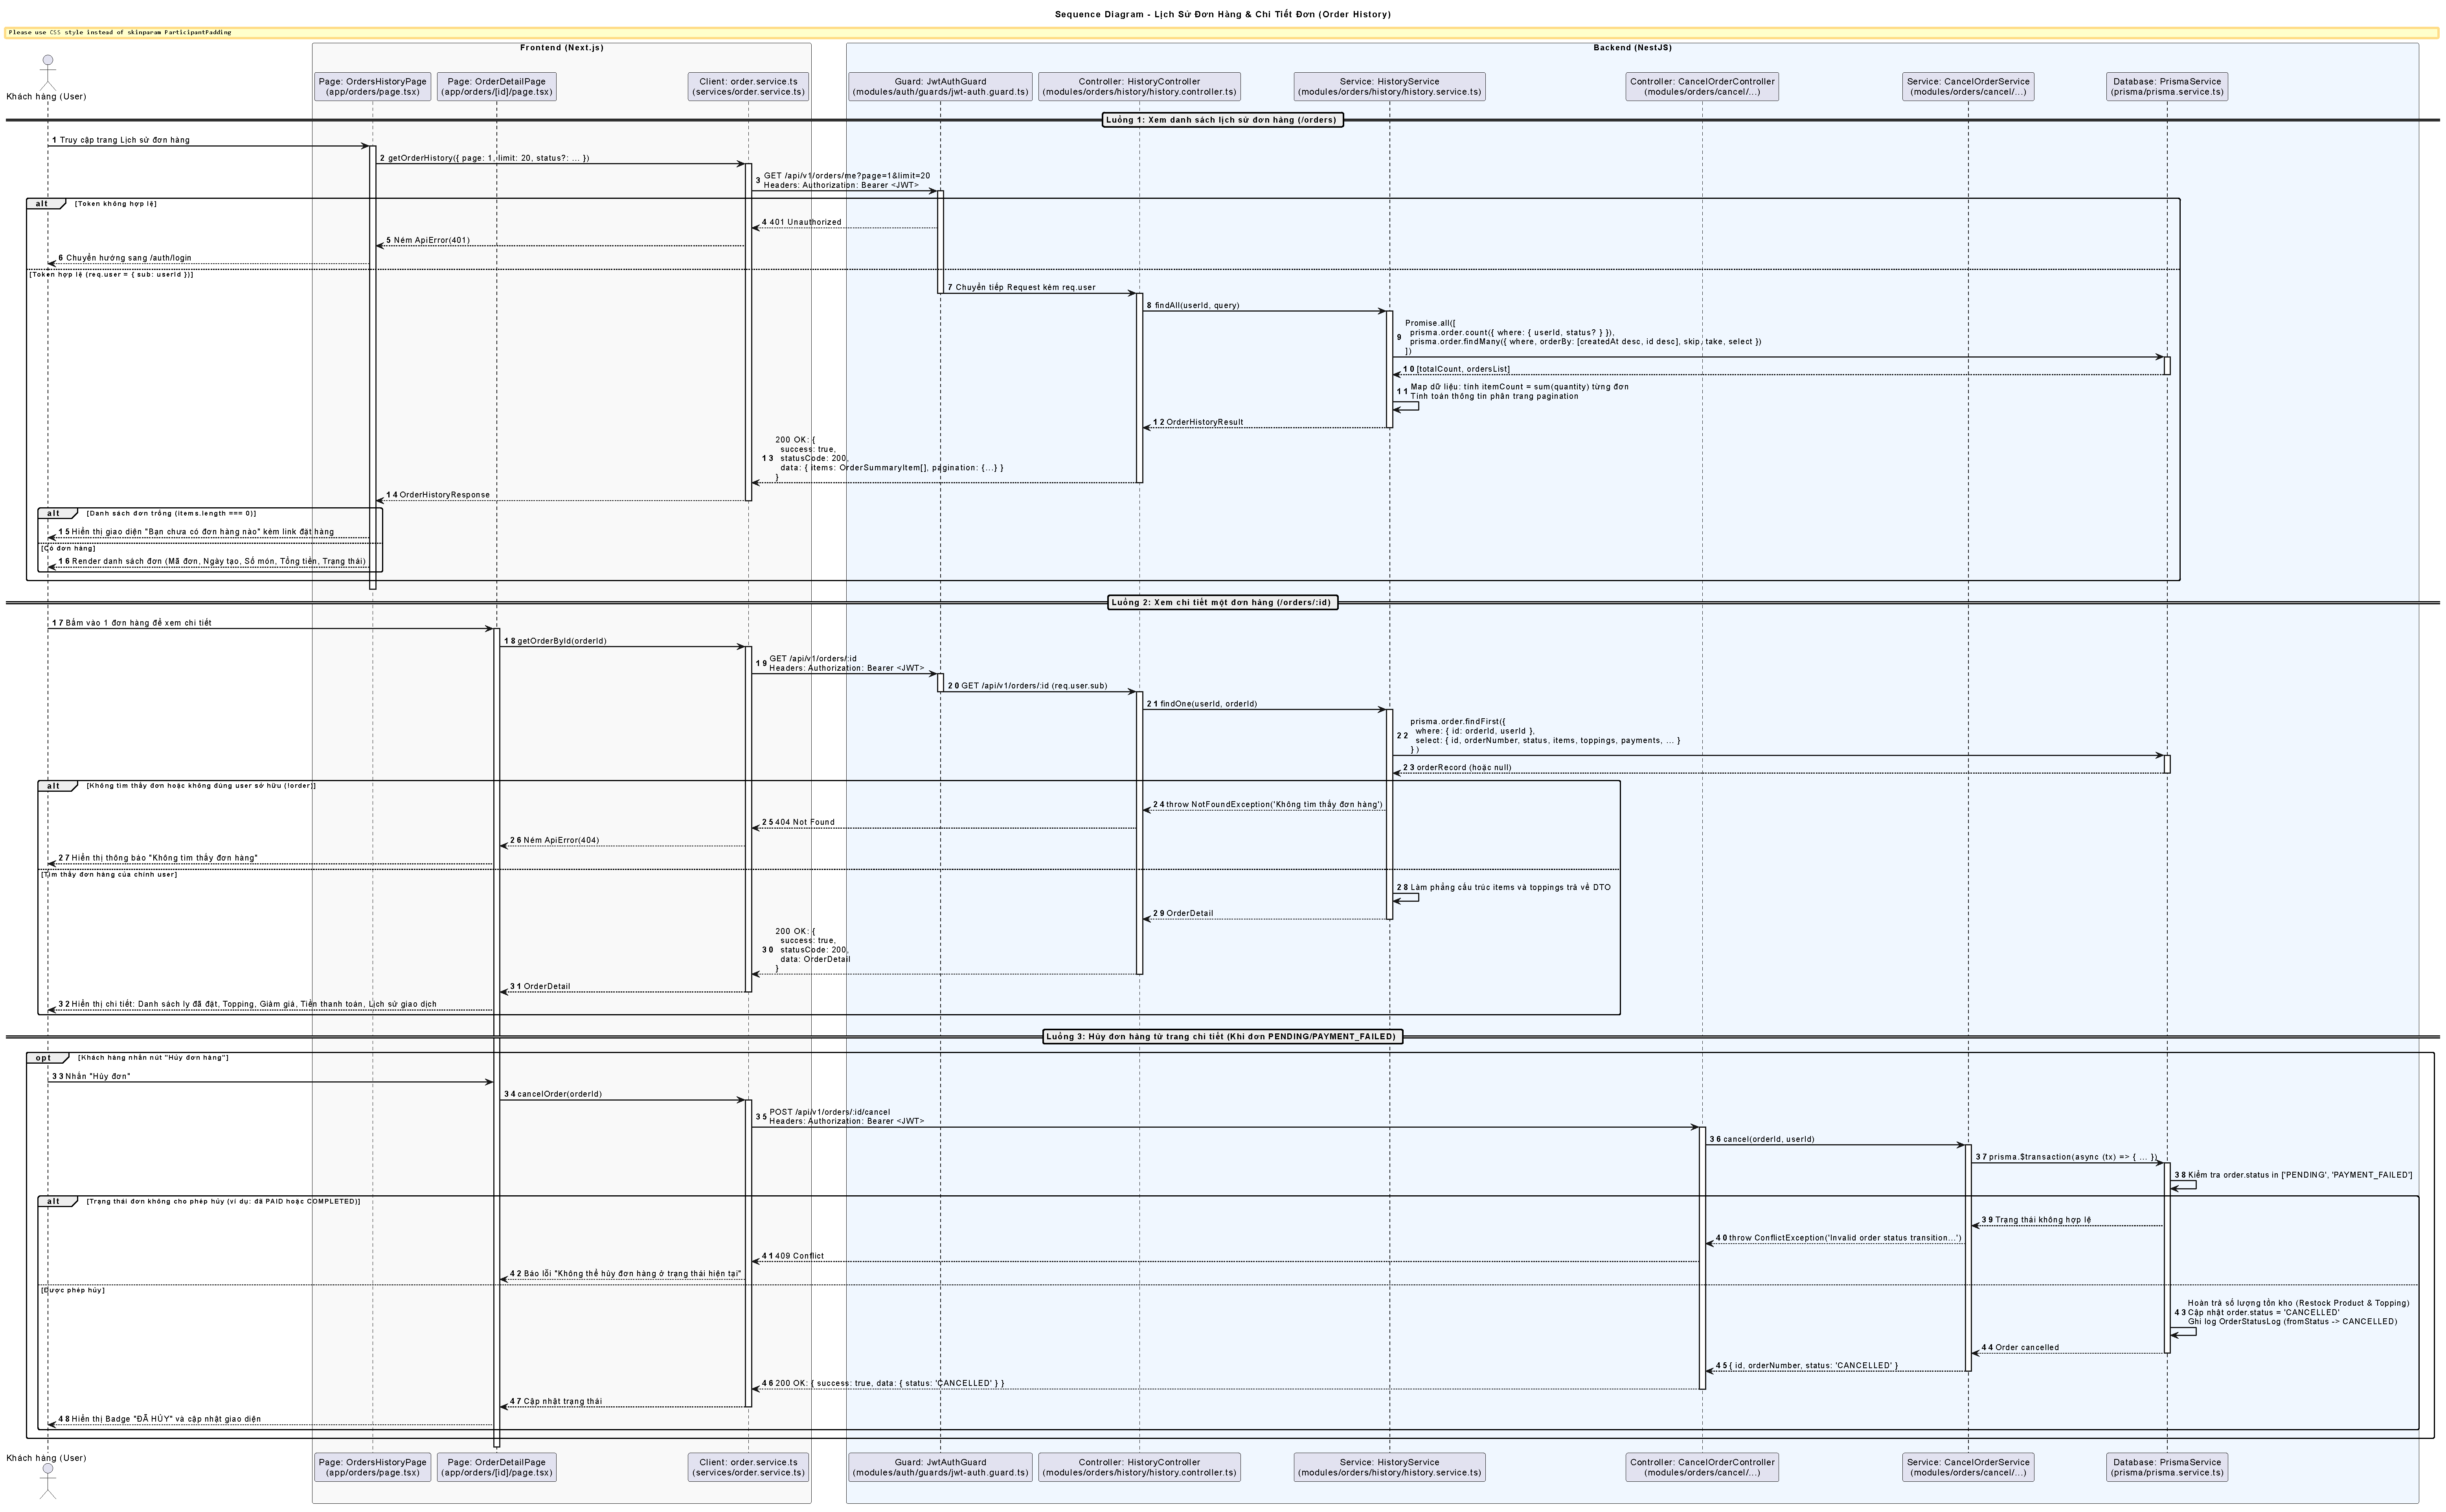
\includegraphics[width=0.9\textwidth]{figures/sequence-order-history.pdf}
    \caption{Sơ đồ Tuần tự - Phân hệ Lịch sử Đơn hàng}
    \label{fig:sequence-order-history}
\end{figure}

\subsection{Hợp đồng API (API Contract)}
\begin{table}[htbp]
\centering
\small
\caption{Danh mục API Endpoints - Phân hệ Lịch sử Đơn hàng}
\label{tab:api-history}
\begin{tabularx}{\textwidth}{llp{4cm}X}
\toprule
\textbf{Phương thức} & \textbf{Endpoint} & \textbf{Header} & \textbf{Phản hồi chính} \\
\midrule
\texttt{GET} & \texttt{/api/v1/orders} & \texttt{Authorization: Bearer <JWT>} & \texttt{200 OK}: Danh sách các đơn hàng của user đang đăng nhập, kèm tổng tiền và trạng thái. \\
\texttt{GET} & \texttt{/api/v1/orders/:id} & \texttt{Authorization: Bearer <JWT>} & \texttt{200 OK}: Chi tiết đơn hàng gồm các món (\texttt{items}), topping và lịch sử trạng thái (\texttt{statusHistory}). Lỗi \texttt{404} nếu không tìm thấy hoặc không thuộc sở hữu. \\
\bottomrule
\end{tabularx}
\end{table}

\subsection{Ánh xạ Cơ sở dữ liệu (Database Mapping)}
\begin{itemize}
    \item Truy vấn danh sách đơn hàng cá nhân:
    \begin{lstlisting}[language=SQL]
SELECT id, order_number, status, total_amount, discount_amount, final_amount, created_at 
FROM orders 
WHERE user_id = :userId 
ORDER BY created_at DESC;
    \end{lstlisting}
    \item Tối ưu hóa: Chỉ mục \texttt{@@index([userId])} và \texttt{@@index([status])} trên bảng \texttt{orders} đảm bảo câu truy vấn thực thi với độ phức tạp \(\mathcal{O}(\log N)\), đáp ứng yêu cầu phản hồi nhanh của hệ thống.
\end{itemize}

\subsection{Kịch bản Kiểm thử (Test Cases)}
\begin{table}[htbp]
\centering
\small
\caption{Tóm lược các Ca kiểm thử tiêu biểu - Phân hệ Lịch sử}
\label{tab:tc-history}
\begin{tabularx}{\textwidth}{llp{2.6cm}p{3cm}Xc}
\toprule
\textbf{Mã TC} & \textbf{Loại} & \textbf{Tiền điều kiện} & \textbf{Endpoint / Màn hình} & \textbf{Kết quả mong đợi} & \textbf{Trạng thái} \\
\midrule
\texttt{TC-HIS-API-01} & Hợp lệ & User có 3 đơn hàng & \texttt{GET /orders} & HTTP 200, trả về đủ 3 đơn sắp xếp mới nhất & Chưa chạy \\
\texttt{TC-HIS-API-02} & Bảo mật & Xem đơn của user khác & \texttt{GET /orders/:id} & HTTP 404 hoặc 403, không lộ đơn của người khác & Chưa chạy \\
\texttt{TC-HIS-UI-01} & Giao diện & User chưa có đơn nào & Màn hình \texttt{/orders} & Hiển thị chuỗi "Bạn chưa có đơn hàng nào" & Chưa chạy \\
\texttt{TC-HIS-UI-03} & Giao diện & Đơn đã bị hủy & Danh sách đơn & Hiển thị đúng badge trạng thái "Đã hủy" & Chưa chạy \\
\bottomrule
\end{tabularx}
\end{table}

\subsection{Giao diện Người dùng}
\begin{figure}[htbp]
    \centering
    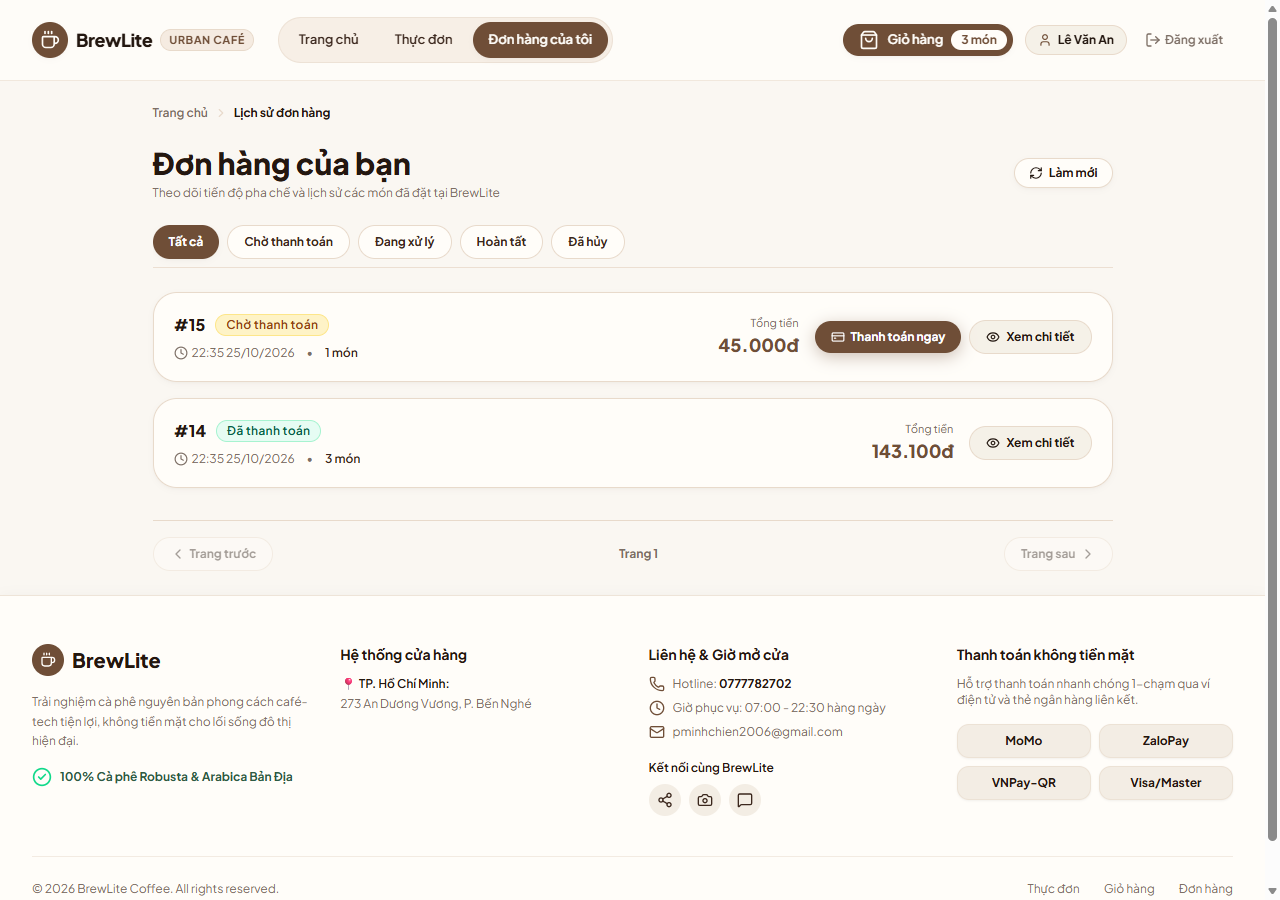
\includegraphics[width=0.92\textwidth]{figures/ui-history.png}
    \caption{Giao diện Lịch sử và Trạng thái Đơn hàng của Khách hàng}
    \label{fig:ui-history}
\end{figure}
